% section
\section{Introduction} \label{section::introduction}
 The thesis will compare different state-of-the-art solutions for image prediction \ref{subsection::imageprediction}.
 The main module, which is a core aspect of this work, is the LSTM (Long short-term memory). \ref{subsection::convlstm}.
 This module was invented by Hochreiter and Schmidhuber  \cite{Hochreiter1997} in 1997 and is used heavily in the field of image prediction since then, e.g. in Srivastave et. al. 
 \cite{Srivastava2015}.
 During the time the module got many different add-ons and changes, which are described in different papers (\cite{Patraucean2015}, \cite{Lotter2016}, \cite{Wang2017}, \cite{Wang2018} and many 
 more.). This work is implementing one specific network architecture (PredNet \cite{Lotter2016}).
 It uses the Shi et. al. \glqq standard\grqq ConvLSTM \cite{Shi2015} as recurrent sub-module, which is changed during the experiments
 with other (more advanced) solutions. The PredNet algorithm is re-implemented in PyTorch \cite{Paszke2019}, as well as the \glqq standard\grqq ConvLSTM and PredRNN.
 Practical experiments are performed on the PredNet using the \glqq standard\grqq ConvLSTM
 and on PredNet using PredRNN instead.
 
 % subsection
 \subsection{Deep Learning} \label{subsection::deeplearning}
 
 % subsection
 \subsection{Image Prediction} \label{subsection::imageprediction}
  Image prediction is a field inside machine learning, where the key is to predict future images, given a sequence of image. The image sequence $X$ is of length $n$, ($x_0, \ldots, x_{n-1}$).
  One possible use-case is the one-frame prediction, where one predicts $x_n$, given the the sequence $X$. Another common use-case is multi-frame prediction, where the key is to predict $t$ many
  frames into the future. This is often performed using sequence-to-sequence learning \cite{Sutskever2014}. Obviously the first frames look much better then the last frames, as ground-truth is 
  missing, and the predicted frames are approximated, which means they contain a certain level of error.

 % subsection
 \subsection{Autoencoder} \label{subsection::autoencoder}

 % subsection
 \subsection{RNN} \label{subsection::rnn}
  RNN (Recurrent neural network)
 
 % subsection
 \subsection{LSTM} \label{subsection::lstm}
  LSTM (Long Short-term Memory) \cite{Hochreiter1997} is a form of RNN, which avoids a critical problem of standard RNN: Saving \textbf{Long-term dependencies} \cite{Goodfellow2016}.
  The architecture consists of different submodules, an inpute-gate, forget-gate, cell-state and output-gate.
  \begin{equation}
   i_t = \sigma(w_{x_i}x_t + w_{h_i}h_{t-1} + w_{c_i}c_{t-1} + b_i)
  \end{equation}
  \begin{equation}
   f_t = \sigma(w_{x_f}x_t + w_{h_f}h_{t-1} + w_{c_f}c_{t-1} + b_f)
  \end{equation}
  \begin{equation}
   c_t = f_tc_{t-1} + i_ttanh(w_{x_c}x_t + w_{h_c}h_{t-1} + b_c)
  \end{equation}
  \begin{equation}
   o_t = \sigma(w_{x_o}x_t + w_{h_o}h_{t-1} + w_{c_o}c_t + b_o)
  \end{equation}
  \begin{equation}
   h_t = o_ttanh(c_t)
  \end{equation}
  $w$ is the weight of the layer, $\sigma$ the sigmoid function, $b$ the layer bias. $h_t$ is the output, in RNN's
  the output is often denoted as hidden.
  \begin{figure}[H]
   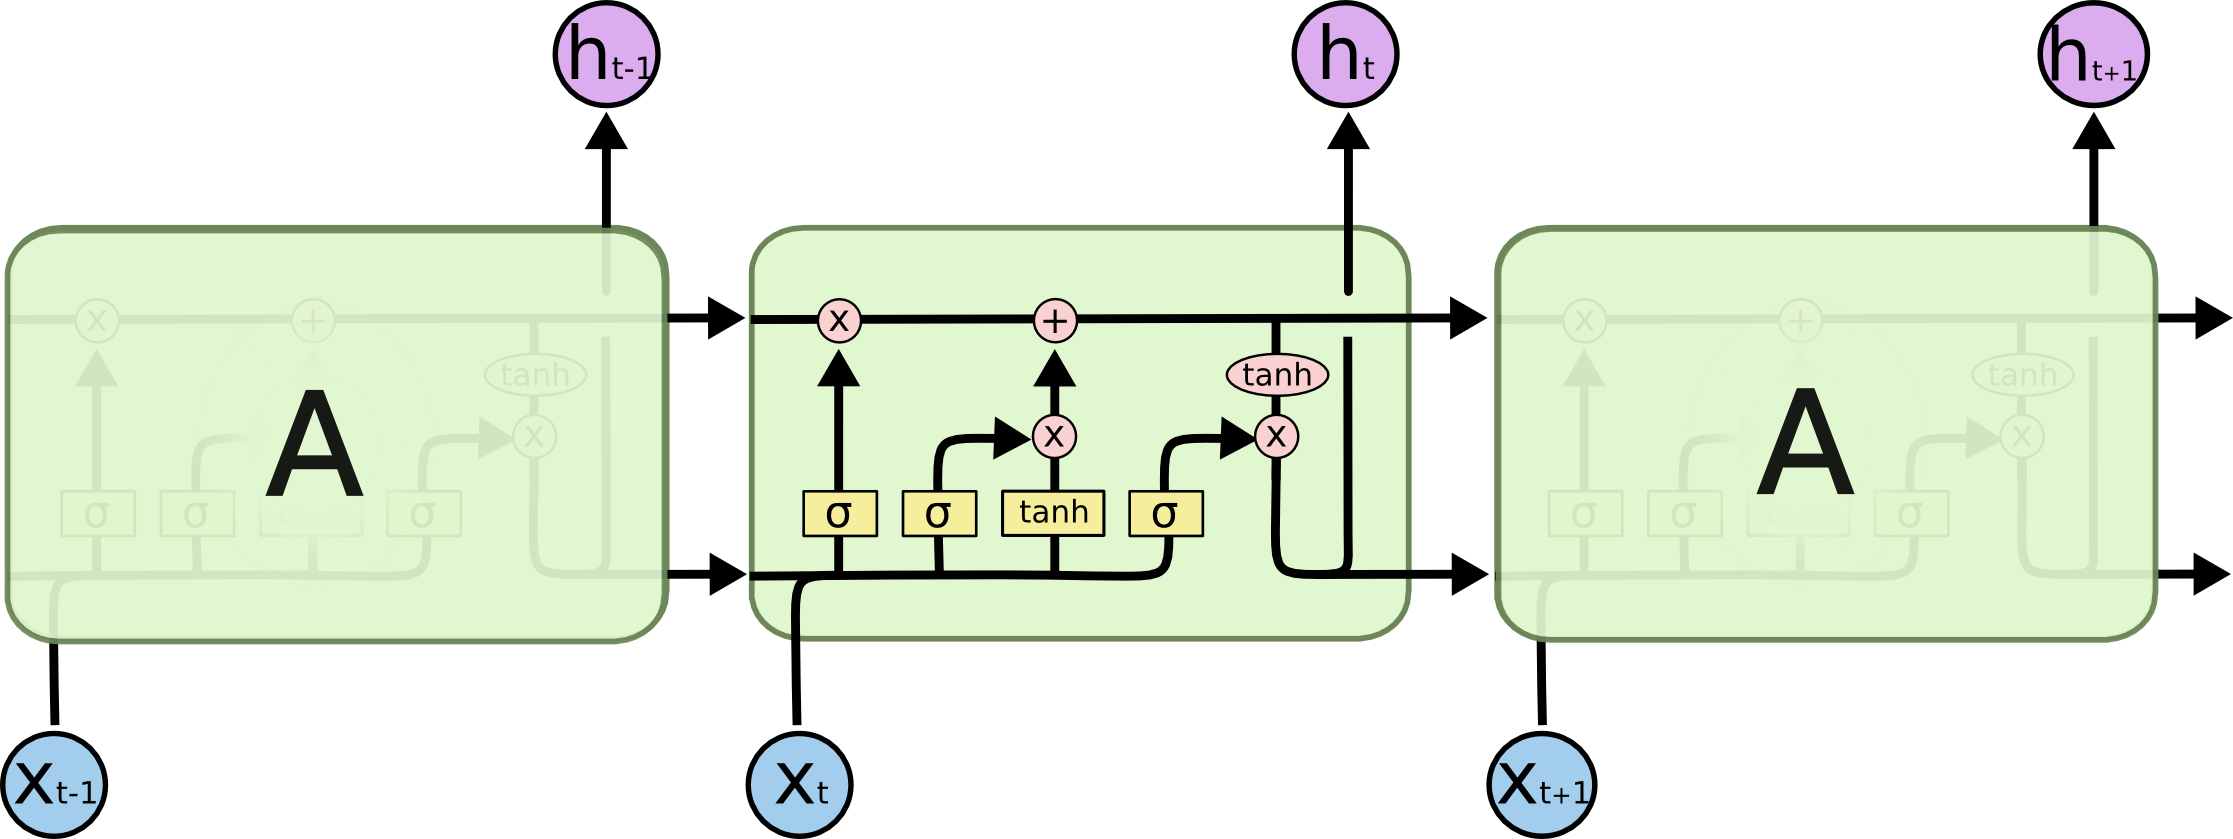
\includegraphics[width=0.6\textwidth]{../Images/lstm_chain.png}
   \centering
   \caption{LSTM Architecture \citep{Olah2015}}
   \label{fig:lstm_architecture}
  \end{figure}
 
 % subsection
 \subsection{ConvLSTM} \label{subsection::convlstm}
  The convolutional LSTM, invented by Shi et. al. \cite{Shi2015} is a LSTM using convolutional layer instead of fully connected ones. Therefore the formulas looks very similar to the ones in    
  section~\ref{subsection::lstm}.
  \begin{equation}
   i_t = \sigma(x_t \ast w_{x_i} + h_{t-1} \ast w_{h_i} + w_{i_b})
  \end{equation}
  \begin{equation}
   f_t = \sigma(x_t \ast w_{x_f} + h_{t-1} \ast w_{h_f} + w_{f_b})
  \end{equation}
  \begin{equation}
   \tilde{c_t} = tanh(x_t \ast w_{x_{\tilde{c}}} + h_{t-1} \ast w_{h_{\tilde{c}}} + w_{c_{\tilde{b}}})
  \end{equation}
  \begin{equation}
   c_t = \tilde{c_t} \odot i_t + c_{t-1} \odot f_t
  \end{equation}
  \begin{equation}
   o_t = \sigma(x_t \ast w_{x_o} + h_{t-1} \ast w_{h_o} + w_{o_b})
  \end{equation}
  \begin{equation}
   h_t = o_t \odot tanh(c_t)
  \end{equation}
  $\ast$ is the commonly used sign for the convolution operation.\\
  $\odot$ is the hadamard product (point-wise multiplication).
  
 % subsection
 \subsection{PyTorch} \label{subsection::pytorch}